\documentclass[]{article}
\usepackage{lmodern}
\usepackage{amssymb,amsmath}
\usepackage{ifxetex,ifluatex}
\usepackage{fixltx2e} % provides \textsubscript
\ifnum 0\ifxetex 1\fi\ifluatex 1\fi=0 % if pdftex
  \usepackage[T1]{fontenc}
  \usepackage[utf8]{inputenc}
\else % if luatex or xelatex
  \ifxetex
    \usepackage{mathspec}
  \else
    \usepackage{fontspec}
  \fi
  \defaultfontfeatures{Ligatures=TeX,Scale=MatchLowercase}
\fi
% use upquote if available, for straight quotes in verbatim environments
\IfFileExists{upquote.sty}{\usepackage{upquote}}{}
% use microtype if available
\IfFileExists{microtype.sty}{%
\usepackage[]{microtype}
\UseMicrotypeSet[protrusion]{basicmath} % disable protrusion for tt fonts
}{}
\PassOptionsToPackage{hyphens}{url} % url is loaded by hyperref
\usepackage[unicode=true]{hyperref}
\hypersetup{
            pdfborder={0 0 0},
            breaklinks=true}
\urlstyle{same}  % don't use monospace font for urls
\usepackage{longtable,booktabs}
% Fix footnotes in tables (requires footnote package)
\IfFileExists{footnote.sty}{\usepackage{footnote}\makesavenoteenv{long table}}{}
\usepackage{graphicx,grffile}
\makeatletter
\def\maxwidth{\ifdim\Gin@nat@width>\linewidth\linewidth\else\Gin@nat@width\fi}
\def\maxheight{\ifdim\Gin@nat@height>\textheight\textheight\else\Gin@nat@height\fi}
\makeatother
% Scale images if necessary, so that they will not overflow the page
% margins by default, and it is still possible to overwrite the defaults
% using explicit options in \includegraphics[width, height, ...]{}
\setkeys{Gin}{width=\maxwidth,height=\maxheight,keepaspectratio}
\IfFileExists{parskip.sty}{%
\usepackage{parskip}
}{% else
\setlength{\parindent}{0pt}
\setlength{\parskip}{6pt plus 2pt minus 1pt}
}
\setlength{\emergencystretch}{3em}  % prevent overfull lines
\providecommand{\tightlist}{%
  \setlength{\itemsep}{0pt}\setlength{\parskip}{0pt}}
\setcounter{secnumdepth}{0}
% Redefines (sub)paragraphs to behave more like sections
\ifx\paragraph\undefined\else
\let\oldparagraph\paragraph
\renewcommand{\paragraph}[1]{\oldparagraph{#1}\mbox{}}
\fi
\ifx\subparagraph\undefined\else
\let\oldsubparagraph\subparagraph
\renewcommand{\subparagraph}[1]{\oldsubparagraph{#1}\mbox{}}
\fi

% set default figure placement to htbp
\makeatletter
\def\fps@figure{htbp}
\makeatother


\date{}

\begin{document}

{Trabajo Práctico Computacional}

{}

{Estructura de la Materia 3}

{Departamento de Física}

{Facultad de Ciencias Exactas y Naturales}

{Universidad de Buenos Aires}

{}

{}

{}

{}

{}

{}

{}

{}

{}

{}

{}

{}

{}

{}

{}

{}

{}

{}

{}

{}

{}

{}

{}

{Integrantes}

{Rosa María Sandá}

{Sebastián Schiavinato}

\begin{center}\rule{0.5\linewidth}{\linethickness}\end{center}

{Introducción. Información experimental}

{El objetivo de este trabajo fue hacer un estudio de la molécula de
ácido sulfhídrico, también conocida como sulfuro de hidrógeno (H}{2}{S),
utilizando una serie de métodos computacionales estándares en la física
molecular. Este estudio abarca la determinación de su multiplicidad,
geometría de equilibrio, potencial de ionización, energía del estado
fundamental, así como el análisis de sus orbitales moleculares y
naturales y su disociación.}

{El H}{2}{S cuenta con 18 electrones (16 del S y 1 de cada H) y ~tiene
carga 0 (neutra). La distancia entre el S y cada uno de los ~H es
idéntica, e igual a 1,336 Å, y el ángulo H-S-H es de 92,11º. El dipolo
experimental es de 0,970 Debye.}

{Esta molécula tiene una geometría simétrica que verifica el grupo
puntual C}{2v}{, que corresponde a tener dos planos de simetría
verticales y una rotación en el eje formado por los dos planos en 180º.
Esta simetría se puede observar en la Figura 1. A partir de estas
operaciones de simetría se deduce la igualdad de las distancias entre S
y los H, además de la existencia de un solo grado de libertad más, el
ángulo entre H-S-H.}

{}

{Desarrollo experimental y resultados}

{}

{Determinación de la multiplicidad de espín del estado fundamental}

{~~~~~~~~Para determinar la multiplicidad de espín de la molécula
H}{2}{S, utilizando el }{Gaussian }{03W}{~}{se realizaron ~cálculos de
Hartree Fock restricto (RHF) e irrestricto (UHF), utilizando a su vez
dos multiplicidades distintas: 1(singlete) y 3 (triplete). Se ~utilizó
en todos los casos la base STO-3G y los datos experimentales para la
geometría. Cabe ~aclarar que para el caso triplete, el Hartree Fock
restricto realizado fue de capa abierta (ROHF), para romper con la
condición de orbitales doblemente ocupados (que sólo puede dar una
configuración singlete).}

{A partir de buscar la energía mínima entre las obtenidas para el estado
fundamental de la molécula en cada caso (ver Tabla 1), se pudo
determinar que la molécula del H}{2}{S ~es un singlete (s=0), resultado
que se corrobora con los datos experimentales. Asimismo, la energía en
este caso no sólo resultó mínima, sino que se pudo verificar que resultó
~igual para los dos métodos utilizados (RHF y UHF).}

{}

{Optimización de geometría}

{~~~~~~~~Una vez determinada la multiplic}{idad ~del H}{2}{S (necesaria
para los cálculos con el }{Gaussian 03W}{), se procedió en primera
instancia a hacer una optimización de la geometría de la molécula,
usando a su vez el método}{~}{RHF con una base STO-3G. Como geometría
inicial para hacer la optimización de la misma, se propuso una que
respetara la simetría experimental de la molécula (con el átomo de
azufre como origen de coordenadas, y los átomos de hidrógeno }{en un
mismo plano, a igual distancia del azufre}{). La matriz de las
coordenadas de cada uno de los átomos obtenida se observa
comparativamente con la experimental en la Tabla 2. Nótese que la
optimización respeta la simetría propuesta para la molécula, y las
coordenadas de las posiciones de los átomos son muy parecidas en valor
absoluto a las experimentales (difieren en menos de 0.1 Å). Notando a su
vez lo difícil de hacer comparaciones viendo de forma directa la
posición de los átomos, se decidió calcular el valor cuadrático medio
(RMS) de las diferencias entre las posiciones de cada átomo obtenidas
numéricamente y las dadas por los datos experimentales. }

{~~~~~~~~La optimización utilizando el método RHF se probó en otras
bases más grandes (6-31G, 6-31G**, cc-pVDZ y cc-pVTZ), utilizando como
geometría inicial la obtenida en la optimización previa. Los resultados
de la energía del estado fundamental para la geometría optimizada en
cada caso, así como el valor RMS previamente detallado, se observan en
la Tabla 3. Se pudo verificar cómo al ir aumentando el tamaño de la
base, la energía fue disminuyendo, hasta alcanzar un mínimo para la base
cc-pVTZ. Además se observa una particular deficiencia en el cálculo
utilizando la base STO-3G (la energía con esta base resultó
sorpresivamente 4 E}{h}{~más alta que la obtenida con las bases más
grandes), que se puede explicar asumiendo que la base tiene muy pocos
elementos para describir a la molécula. Con las mismas bases se
repitieron los cálculos con el método de UHF, ~y se obtuvieron
exactamente los mismos resultados que con RHF.}

{~~~~~~~~Considerando que el tiempo de cómputo aumentó considerablemente
al utilizar la base cc-pVTZ, se decidió que la base óptima para los
cálculos era la cc-pVDZ (teniendo en cuenta la relación costo
computacional/resultados). Con esta base, se procedió a hacer nuevamente
la optimización con otros métodos: CID, CISD y B3LYP. En los resultados
(ver Tabla 3), se observa que la energía más baja tras la optimización
fue la obtenida para el método DFT (B3LYP), casi 1 E}{h}{~inferior que
las obtenidas con todos los otros métodos, pero este resultado debe
leerse con cuidado si se tiene en cuenta que los métodos DFT no respetan
el principio variacional, por lo que podría tratarse de una energía por
debajo de la energía del estado fundamental real. En cuanto a los dos
métodos de configuración de interacciones, se puede apreciar la mejoría
en el cálculo al hacer CID y CISD respecto de los métodos RHF/UHF en una
disminución de la energía de los 0.2 E}{h}{. Teniendo en cuenta que al
hacer CISD aumentó el tiempo de cálculo apreciablemente respecto de
hacer CID, se concluye que el método/base óptimos para hacer los
cálculos es el CID/cc-pVDZ, sumado a que fue el método con el que se
obtuvo el menor RMS entre la geometría optimizada y la experimental
(omitiendo el caso RHF/STO-3G, ya discutido y descartado).}

{~~~~~~~~Para todos los métodos, se verificó que las fuerzas sobre los
núcleos (también devueltas por el }{Gaussian 03W}{), tienden a cero
cerca de la geometría convergida (e iban disminuyendo con cada paso de
la iteración). Asimismo, como las frecuencias vibracionales obtenidas en
todos los casos son reales (ver Tabla 3), podemos afirmar que las
geometrías halladas son ~estables.}

{~~~~~~~~}

{Orbitales moleculares}

{Para poder visualizar los orbitales moleculares del H}{2}{S, se realizó
un cálculo RHF usando la base 3-21G. Se optó por utilizar los datos
experimentales para la geometría de la molécula. Utilizando la base
mencionada, se obtuvieron 17 orbitales moleculares en total, 9 de los
cuales estaban doblemente ocupados por los 18 electrones de la molécula.
Los energías de los 9 orbitales ocupados resultaron todas menores a cero
y no degeneradas (ver Tabla }{4}{). ~El gap de energía entre el HOMO
(orbital 9) y el LUMO (orbital 10) resultó de 0}{,}{57 E}{h}{~}{~(a dos
cifras significativas). }

{Utilizando el }{GaussView}{, se graficaron los orbitales moleculares
ocupados y el LUMO. Los mismos pueden observarse en la Figura 2, donde
no se incluyen los orbitales moleculares 1 y 2 (los de más baja
energía), por ser orbitales de core centrados en el átomo de azufre. A
partir de los mismos, puede verificarse que el orbital molecular HOMO
sólo tiene contribuciones de los orbitales atómicos del azufre, y que el
orbital LUMO incluye contribuciones de los orbitales atómicos de tipo s
de los dos Hidrógenos.}

{}

{Determinación de la multiplicidad de espín del estado fundamental de la
molécula}{~simple y doblemente ionizada}

{~~~~~~~~Para determinar la multiplicidad de espín del estado
fundamental de la molécula simplemente ionizada (}{H}{2}{S}{+}{) ~y
doblemente ionizada (}{H}{2}{S}{++}{), se hicieron cálculos ROHF y UHF
con base 3-21G y datos experimentales para la geometría, utilizando a su
vez varias multiplicidades distintas en cada caso, ~acordes al número de
electrones de cada ion (multiplicidades pares para }{H}{2}{S}{+}{, de 17
electrones, y multiplicidades impares para }{H}{2}{S}{++}{, con 16
electrones). ~A partir de las energías obtenidas en cada caso (ver Tabla
}{5}{~y }{6}{), ~se concluye que el }{H}{2}{S}{+}{~es un doblete
(s=}
\includegraphics{images/image1.png}{) y que el }{H}{2}{S}{++}{~}{es
un triplete (s=1).}

{}

{Potencial de ionización}

{~~~~~~~~Una vez determinada la multiplicidad de la molécula ionizada
(}{H}{2}{S}{+}{), se buscó determinar el potencial de ionización d}{el
}{H}{2}{S}{. Para ello, se calculó utilizando distintos métodos la
energía del estado fundamental para el ~}{H}{2}{S}{+}{~}{~y para el
H}{2}{S y se hizo la diferencia, lo que da la energía de ionización. Los
métodos utilizados fueron RHF (ROHF para el caso de H}{2}{S}{+}{), UHF,
CID, BLYP y BLYP, ~y se usaron a su vez dos bases distintas: 3-21G y
cc-pVDZ. ~En todos los casos se utilizó la geometría experimental de la
molécula. A su vez, se calculó la energía de ionización utilizando el
teorema de Koopman: el potencial de ionización es el módulo de la
energía orbitalaria del H}{O}{MO que se obtiene al hacer RHF en la
molécula H}{2}{S. Para nuestro caso, dicha energía resultó de ~}{0.39
E}{h}{~(a dos cifras significativas). }

{~~~~~~~~Los resultados pueden observarse en la Tabla }{7}{, y si se los
compara con la energía de ionización experimental, de 0.38 E}{h}{~(a dos
cifras significativas), se puede verificar que efectivamente el teorema
de Koopman da una mejor aproximación al potencial de ionización que los
métodos asociados a Hartree Fock (RHF, UHF y CID), ~debido a la
aproximación de orbitales congelados, que pese a no tener
correspondencia con la descripción física del fenómeno (al no tener en
cuenta la nueva relajación del sistema ionizado), compensa el error
asociado a la aproximación de Hartree Fock (que es suponer que el estado
fundamental de cualquier molécula es unideterminantal). Mientras que por
Teorema de Koopman el potencial difiere en 0}{,}{01 E}{h}{~respecto del
experimental, con los métodos de tipo Hartree-Fock el potencial difiere
entre ~los 0}{,}{02 E}{h ~}{hasta los ~0}{,}{05 E}{h}{. ~Por otra parte,
se puede observar ~que los métodos DFT (BLYP y B3LYP), d}{an}{~una
aproximación tan buena como la de Koopman}{, ya}{~que en ambos métodos
(con las dos bases }{utilizadas),}{~la energías de ionización obtenidas
no difieren en más de 0}{,}{01 E}{h ~}{respecto del potencial de
ionización experimental.}

{}

{Orbitales naturales}

{Para visualizar los orbitales naturales, los cuales justifican el uso
de estructuras de Lewis para entender el enlace y la geometría de la
molécula, se partió de los orbitales moleculares obtenidos ~}{~}{del
cálculo RHF en base 3-21g. }

{En la Figura 3 podemos ver los orbitales naturales para la molécula de
H}{2}{S, donde no se grafican los orbitales 1 y 2 ya que son core de
cada átomo y no agregan información relevante a la molécula. Se pueden
ver los orbitales 3, 4 y 5 como orbitales de }{core}{~ubicados en el S,
mientras que los orbitales 6 y 9 son de tipo }{lone pair}{; estos
orbitales se corresponden con los electrones libres de la estructura de
Lewis para la molécula H}{2}{S (ver Figura 2) y están centrados en el S.
Los orbitales 7 y 8 son simétricos y justifican el enlace entre el S y
cada uno de los H. En la Tabla 8 se muestra la ocupación y la energía de
cada orbital.}

{}

{Carga natural y dipolo natural}

{Esta transformación de los orbitales también trae cambios en la
distribución de la carga sobre cada átomo. La carga natural y la carga
Mulliken (que corresponde a la carga deducida en el análisis poblacional
que hace el }{Gaussian 03W)}{~se pueden observar de forma comparativa en
la Tabla 8 . }

{Respecto al dipolo de la molécula H}{2}{S (ver Tabla 9) no se observa
un cambio significativo, aunque ambos dipolos difieren fuertemente del
valor experimental (en casi un factor de 2). Como no se conoce un
principio variacional para el dipolo, estos métodos no necesariamente se
acercarán al valor experimental al aumentar la complejidad de ambos.}

{}

{Disociación de la molécula}

{Por último, se calculó la energía del H}{2}{S en función de la
distancia H-S para varios métodos, manteniendo el ángulo H-S-H
constante, para obtener la curva de energía potencial (PEC). ~En esta
curva se esperó que ~el mínimo fuera alrededor de 1,336 Å (valor
experimental de equilibrio), así como se esperó que al tender la
distancia al infinito la energía del sistema disociado correspondiera a
la suma de la energía de dos átomos de hidrógeno y uno de azufre, que
corresponde a la disociación real (en tres partes no interactuantes) del
sistema.}

{En la Figura 5 se muestra la disociación para los métodos RHF y UHF,
con la base 6-31G. Se corroboró ~que a partir de los 3Å el método
restricto tiene una mayor energía que el irrestricto, ya que considerar
la misma cantidad de orbitales de tipo α y β agrega una correlación
entre los átomos que no debería existir a largas distancias. Además se
puede observar que la distancia de equilibrio experimental está en la
zona de equilibrio de la molécula, lo que recupera el resultado de
optimización que ya se había efectuado. }{Ni el método RHF ni el UHF
describen correctamente la energía en el infinito, con lo que queda
demostrado}{~que el método sigue correlacionando los átomos aún
~prácticamente ~en el infinito (más de 2 veces la distancia de
equilibrio).}

{Para comparar se repitió el cálculo con el método B3LYP en la base
cc-pVDZ (para mejorar la convergencia), el cual puede verse en la Figura
6, y ~nuevamente se ve la diferencia entre el caso irrestricto y
restricto. El punto de la curva donde se separan ambos casos es
diferente al caso de Hartree Fock, lo que expone que esta diferencia no
es simplemente producto de usar el caso restricto o irrestricto sino
también depende del método computacional utilizado}{. El método UB3LYP
tiene una energía en el infinito muy parecida al valor realmente
disociado, como se ve en la Figura 6, lo que indica que permite
describir mejor el proceso de disociación. }

{Finalmente, en la Figura 7 se observan las curvas de energía potencial
para el caso restricto y los métodos HF, DFT y CISD. Cabe resaltar que
la energía calculada por DFT tiene casi 1 E}{h}{~menos que el resto de
los métodos, lo que podría ser producto que el método no verifica el
principio variacional.}{~}

\begin{center}\rule{0.5\linewidth}{\linethickness}\end{center}

{}

{Anexo}

{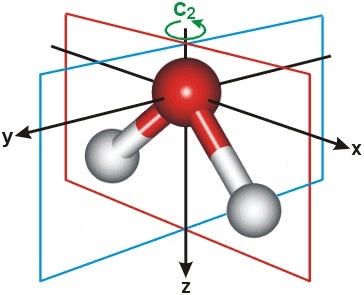
\includegraphics{images/image2.jpg}}

{Figura 1}{~: }{Diagrama del grupo puntual de simetría C}{2v }{de}{~la
molécula ~H}{2}{S (S en rojo y H en blanco).}

{}

\protect\hypertarget{t.b57a46846ece3c15b5863e4cf88b4c3f687eaec1}{}{}\protect\hypertarget{t.0}{}{}

\begin{longtable}[]{@{}lll@{}}
\toprule
\begin{minipage}[t]{0.30\columnwidth}\raggedright\strut
{Multiplicidad}\strut
\end{minipage} & \begin{minipage}[t]{0.30\columnwidth}\raggedright\strut
{Método}\strut
\end{minipage} & \begin{minipage}[t]{0.30\columnwidth}\raggedright\strut
{E}{O}{~(E}{h}{)}\strut
\end{minipage}\tabularnewline
\begin{minipage}[t]{0.30\columnwidth}\raggedright\strut
{1 (singlete)}\strut
\end{minipage} & \begin{minipage}[t]{0.30\columnwidth}\raggedright\strut
{RHF}\strut
\end{minipage} & \begin{minipage}[t]{0.30\columnwidth}\raggedright\strut
{-394,3115553}\strut
\end{minipage}\tabularnewline
\begin{minipage}[t]{0.30\columnwidth}\raggedright\strut
{1 (singlete)}\strut
\end{minipage} & \begin{minipage}[t]{0.30\columnwidth}\raggedright\strut
{UHF}\strut
\end{minipage} & \begin{minipage}[t]{0.30\columnwidth}\raggedright\strut
{-394,3115553}\strut
\end{minipage}\tabularnewline
\begin{minipage}[t]{0.30\columnwidth}\raggedright\strut
{3 (triplete)}\strut
\end{minipage} & \begin{minipage}[t]{0.30\columnwidth}\raggedright\strut
{ROHF}\strut
\end{minipage} & \begin{minipage}[t]{0.30\columnwidth}\raggedright\strut
{-394,0022780}\strut
\end{minipage}\tabularnewline
\begin{minipage}[t]{0.30\columnwidth}\raggedright\strut
{3 (triplete)}\strut
\end{minipage} & \begin{minipage}[t]{0.30\columnwidth}\raggedright\strut
{UHF}\strut
\end{minipage} & \begin{minipage}[t]{0.30\columnwidth}\raggedright\strut
{-394,0070163}\strut
\end{minipage}\tabularnewline
\bottomrule
\end{longtable}

{}

{Tabla 1}{: Energías para el estado fundamental de ~la
molécula}{~}{~H}{2}{S}{~(E}{O}{)}{, obtenidas utilizando diferentes
métodos de Hartree Fock ~y suponiendo dos multiplicidades de espín
distintas. Se usó en todos los casos base STO-3G y la geometría
experimental de la molécula}

{}

{}

\protect\hypertarget{t.0f39b38b2ec5620d8d8d308b10fc169b45aeca1e}{}{}\protect\hypertarget{t.1}{}{}

{}

{Átomo}

{X (Å)}

{Y (Å)}

{Z (Å)}

{Experimental}

{S}

{0}

{0}

{0,1030}

{H(1)}

{0}

{0,9616}

{-0,8239}

{H(2)}

{0}

{-0,9616}

{-0,8239}

{RHF,}

{STO-3G, opt.}

{S}

{0}

{0}

{0,1021}

{H(1)}

{0}

{0,9600}

{-0,8165}

{H(2)}

{0}

{-0,9600}

{-0,8165}

{}

{Tabla 2}{: Geometría experimental para el H}{2}{S y geometría obtenida
haciendo un cálculo de optimización con método RHF y base STO-3G. Las
coordenadas de los átomos ~están dadas en un sistema de ejes cartesianos
X-Y-Z.}

{}

{}

{}

{}

{}

\protect\hypertarget{t.36309b054e1fcb0fbf52c4d3406661b6e91bf8cb}{}{}\protect\hypertarget{t.2}{}{}

{Método}

{Base}

{RMS}

{E}{0}{~(E}{h}{)}

{Frecuencias (A}{1}{,A}{1}{,B}{2}{){[}cm}{-1}{{]}}

{RHF/UHF}

{STO-3G}

{0,006}

{-394,3116301}

{1610, 3274, 3322}

{6-31G}

{0,04}

{-398,6275514}

{2690, 1295, 2717 }

{6-31**}

{0,02}

{-398,6760496}

{2896, 1341, 2864}

{cc-pVDZ}

{0,02}

{-398,6946749}

{2859, 1307, 2872}

{cc-pVTZ}

{0,02}

{-398,7131154}

{2854, 1341, 2908}

{B3LYP}

{cc-pVDZ}

{0,03}

{-399,4097648}

{2672, 1192, 2689}

{CID}

{cc-pVDZ}

{0,01}

{-398,8534621}

{2777, 1237, 2790}

{CISD}

{cc-pVDZ}

{0,02}

{-398,8541566}

{2770, 1236, 2783}

{}

{Tabla 3}{: Energías para el estado fundamental de ~la molécula ~H}{2}{S
(E}{O}{), frecuencias vibracionales y RMS de las diferencias entre las
posiciones de cada átomo obtenidas numéricamente optimizando geometría
~y las dadas por los datos experimentales, con diferentes métodos y
bases. Se destaca en celeste el método/base óptimos teniendo en cuenta
la relación costo computacional/calidad de resultados.}

{}

{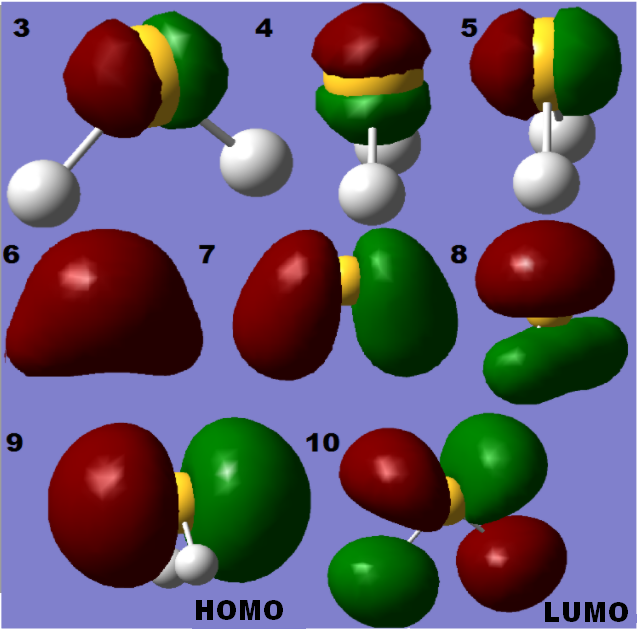
\includegraphics{images/image5.png}}

{Figura 2}{: Orbitales moleculares ocupados (3-9) y orbital molecular
vacante de menor energía (10), obtenidos con }{GaussView}{, utilizando
los resultados del cálculo RHF con base 3-21G para la molécula de
H}{2}{S. Dichos orbitales están numerados en función ~sus energías
orbitalarias (ver Tabla }{4}{).}

{}

{}

{}

\protect\hypertarget{t.0c188b2daf5290b9405efa75cd6eeecd327549b7}{}{}\protect\hypertarget{t.3}{}{}

\begin{longtable}[]{@{}llll@{}}
\toprule
\begin{minipage}[t]{0.22\columnwidth}\raggedright\strut
{OM}\strut
\end{minipage} & \begin{minipage}[t]{0.22\columnwidth}\raggedright\strut
{E. orbitalaria (E}{h}{)}\strut
\end{minipage} & \begin{minipage}[t]{0.22\columnwidth}\raggedright\strut
{OM}\strut
\end{minipage} & \begin{minipage}[t]{0.22\columnwidth}\raggedright\strut
{E. orbitalaria (E}{h}{)}\strut
\end{minipage}\tabularnewline
\begin{minipage}[t]{0.22\columnwidth}\raggedright\strut
{1}\strut
\end{minipage} & \begin{minipage}[t]{0.22\columnwidth}\raggedright\strut
{-91,31955}\strut
\end{minipage} & \begin{minipage}[t]{0.22\columnwidth}\raggedright\strut
{6}\strut
\end{minipage} & \begin{minipage}[t]{0.22\columnwidth}\raggedright\strut
{-1,00328}\strut
\end{minipage}\tabularnewline
\begin{minipage}[t]{0.22\columnwidth}\raggedright\strut
{2}\strut
\end{minipage} & \begin{minipage}[t]{0.22\columnwidth}\raggedright\strut
{-8,92265}\strut
\end{minipage} & \begin{minipage}[t]{0.22\columnwidth}\raggedright\strut
{7}\strut
\end{minipage} & \begin{minipage}[t]{0.22\columnwidth}\raggedright\strut
{-0,59226}\strut
\end{minipage}\tabularnewline
\begin{minipage}[t]{0.22\columnwidth}\raggedright\strut
{3}\strut
\end{minipage} & \begin{minipage}[t]{0.22\columnwidth}\raggedright\strut
{-6,59767}\strut
\end{minipage} & \begin{minipage}[t]{0.22\columnwidth}\raggedright\strut
{8}\strut
\end{minipage} & \begin{minipage}[t]{0.22\columnwidth}\raggedright\strut
{-0,4939}\strut
\end{minipage}\tabularnewline
\begin{minipage}[t]{0.22\columnwidth}\raggedright\strut
{4}\strut
\end{minipage} & \begin{minipage}[t]{0.22\columnwidth}\raggedright\strut
{-6,59584}\strut
\end{minipage} & \begin{minipage}[t]{0.22\columnwidth}\raggedright\strut
{9}\strut
\end{minipage} & \begin{minipage}[t]{0.22\columnwidth}\raggedright\strut
{-0,39279}\strut
\end{minipage}\tabularnewline
\begin{minipage}[t]{0.22\columnwidth}\raggedright\strut
{5}\strut
\end{minipage} & \begin{minipage}[t]{0.22\columnwidth}\raggedright\strut
{-6,59227}\strut
\end{minipage} & \begin{minipage}[t]{0.22\columnwidth}\raggedright\strut
{10}\strut
\end{minipage} & \begin{minipage}[t]{0.22\columnwidth}\raggedright\strut
{0,18106}\strut
\end{minipage}\tabularnewline
\bottomrule
\end{longtable}

{}

{Tabla 4}{: Energías orbitalarias para los orbitales moleculares (OM)
ocupados (1-9), y el orbital vacante de menor energía (10), obtenidos
del cálculo RHF con base 3-21G para la molécula de H}{2}{S. Se resalta
en color celeste el orbital HOMO (9) y el LUMO (10).}

{}

\protect\hypertarget{t.0d6cdc5d95ba285b548b869a4764ccb9b699afd0}{}{}\protect\hypertarget{t.4}{}{}

\begin{longtable}[]{@{}lll@{}}
\toprule
\begin{minipage}[t]{0.30\columnwidth}\raggedright\strut
{Multiplicidad}\strut
\end{minipage} & \begin{minipage}[t]{0.30\columnwidth}\raggedright\strut
{Método}\strut
\end{minipage} & \begin{minipage}[t]{0.30\columnwidth}\raggedright\strut
{E}{O}{+}{(E}{h}{)}\strut
\end{minipage}\tabularnewline
\begin{minipage}[t]{0.30\columnwidth}\raggedright\strut
{2 (doblete)}\strut
\end{minipage} & \begin{minipage}[t]{0.30\columnwidth}\raggedright\strut
{ROHF}\strut
\end{minipage} & \begin{minipage}[t]{0.30\columnwidth}\raggedright\strut
{-396,3477957}\strut
\end{minipage}\tabularnewline
\begin{minipage}[t]{0.30\columnwidth}\raggedright\strut
{2 (doblete)}\strut
\end{minipage} & \begin{minipage}[t]{0.30\columnwidth}\raggedright\strut
{UHF}\strut
\end{minipage} & \begin{minipage}[t]{0.30\columnwidth}\raggedright\strut
{-396,3494201}\strut
\end{minipage}\tabularnewline
\begin{minipage}[t]{0.30\columnwidth}\raggedright\strut
{4 (cuartete)}\strut
\end{minipage} & \begin{minipage}[t]{0.30\columnwidth}\raggedright\strut
{ROHF}\strut
\end{minipage} & \begin{minipage}[t]{0.30\columnwidth}\raggedright\strut
{-396,0279275}\strut
\end{minipage}\tabularnewline
\begin{minipage}[t]{0.30\columnwidth}\raggedright\strut
{4 (cuartete)}\strut
\end{minipage} & \begin{minipage}[t]{0.30\columnwidth}\raggedright\strut
{UHF}\strut
\end{minipage} & \begin{minipage}[t]{0.30\columnwidth}\raggedright\strut
{-396,0294191}\strut
\end{minipage}\tabularnewline
\bottomrule
\end{longtable}

{}

{Tabla 5}{: Energías para el estado fundamental del catión
H}{2}{S}{+}{~}{(E}{O}{+}{), obtenidas utilizando diferentes métodos de
Hartree Fock ~y suponiendo dos multiplicidades de espín distintas. Se
usó en todos los casos base 3-21G y la geometría experimental de la
molécula.}

{}

\protect\hypertarget{t.173ef4e9e36680a46bb8d829c30c2e3f8bde39e9}{}{}\protect\hypertarget{t.5}{}{}

\begin{longtable}[]{@{}lll@{}}
\toprule
\begin{minipage}[t]{0.30\columnwidth}\raggedright\strut
{Multiplicidad}\strut
\end{minipage} & \begin{minipage}[t]{0.30\columnwidth}\raggedright\strut
{Método}\strut
\end{minipage} & \begin{minipage}[t]{0.30\columnwidth}\raggedright\strut
{E}{O}{++}{~(E}{h}{)}\strut
\end{minipage}\tabularnewline
\begin{minipage}[t]{0.30\columnwidth}\raggedright\strut
{1 (singlete)}\strut
\end{minipage} & \begin{minipage}[t]{0.30\columnwidth}\raggedright\strut
{ROHF}\strut
\end{minipage} & \begin{minipage}[t]{0.30\columnwidth}\raggedright\strut
{-395,5738373}\strut
\end{minipage}\tabularnewline
\begin{minipage}[t]{0.30\columnwidth}\raggedright\strut
{1 (singlete)}\strut
\end{minipage} & \begin{minipage}[t]{0.30\columnwidth}\raggedright\strut
{UHF}\strut
\end{minipage} & \begin{minipage}[t]{0.30\columnwidth}\raggedright\strut
{-395,5738373}\strut
\end{minipage}\tabularnewline
\begin{minipage}[t]{0.30\columnwidth}\raggedright\strut
{3 (triplete)}\strut
\end{minipage} & \begin{minipage}[t]{0.30\columnwidth}\raggedright\strut
{ROHF}\strut
\end{minipage} & \begin{minipage}[t]{0.30\columnwidth}\raggedright\strut
{-395,5760448}\strut
\end{minipage}\tabularnewline
\begin{minipage}[t]{0.30\columnwidth}\raggedright\strut
{3 (triplete)}\strut
\end{minipage} & \begin{minipage}[t]{0.30\columnwidth}\raggedright\strut
{UHF}\strut
\end{minipage} & \begin{minipage}[t]{0.30\columnwidth}\raggedright\strut
{-395,5773692}\strut
\end{minipage}\tabularnewline
\begin{minipage}[t]{0.30\columnwidth}\raggedright\strut
{5 (quintuplete)}\strut
\end{minipage} & \begin{minipage}[t]{0.30\columnwidth}\raggedright\strut
{UHF}\strut
\end{minipage} & \begin{minipage}[t]{0.30\columnwidth}\raggedright\strut
{-395,1910708}\strut
\end{minipage}\tabularnewline
\bottomrule
\end{longtable}

{}

{Tabla 6}{: Energías para el estado fundamental del catión
H}{2}{S}{+}{~(E}{O}{++}{), obtenidas utilizando diferentes métodos de
Hartree Fock ~y suponiendo dos multiplicidades de espín distintas. Se
usó en todos los casos base 3-21G y la geometría experimental de la
molécula.}

{}

{}

\protect\hypertarget{t.0ed4ce1ba2e6be1944273c7a7a2da429623ab111}{}{}\protect\hypertarget{t.6}{}{}

{Método}

{Base}

{E}{O}{~(E}{h}{)}

{E}{O}{+ }{(E}{h}{)}

{IP(E}{h}{)}

{RHF/ROHF}

{3-21G}

{-396,7039571}

{-396,3477957}

{0,36}

{UHF}

{3-21G}

{-396,7039571}

{-396,3494201}

{0,35}

{cc-pVDZ}

{-398,6945414}

{-398,3556018}

{0,34}

{BLYP}

{3-21G}

{-397,3804558}

{-396,9989329}

{0,38}

{cc-pVDZ}

{-399,3790354}

{-399,0051823}

{0,37}

{B3LYP}

{3-21G}

{-397,4124927}

{-397,0227261}

{0,39}

{cc-pVDZ}

{-399,4092724}

{-399,028500}

{0,38}

{CID}

{3-21G}

{-396,7039571}

{-396,3494212}

{0,35}

{cc-pVDZ}

{-398,6945416}

{-398,3556083}

{0,34}

{Koopman}

{3-21 G/ RHF}

{0,39}

{Experimental}

{}

{0,38}

{}

{Tabla 7}{: Potencial de ionización calculador a partir de la diferencia
entre la energías del estado fundamental del catión
H}{2}{S}{+}{~(E}{O}{+}{) y ~de la molécula neutra ~H}{2}{S (E}{O}{),
calculadas a su vez con distintas bases y métodos, usando la geometría
experimental de la molécula. Se incluye además el potencial de
ionización calculado por teorema de Koopman (sacado de la energía
orbitalaria del HUMO del cálculo RHF para el H}{2}{S con base 3-21G), y
el valor experimental de forma comparativa (todos con dos cifras
significativas).}

{\includegraphics{images/image8.gif}}

{Figura 3:}{~Estructura de Lewis del H}{2}{S. Obtenida del applet
https://goo.gl/fFnA5M}

{}

{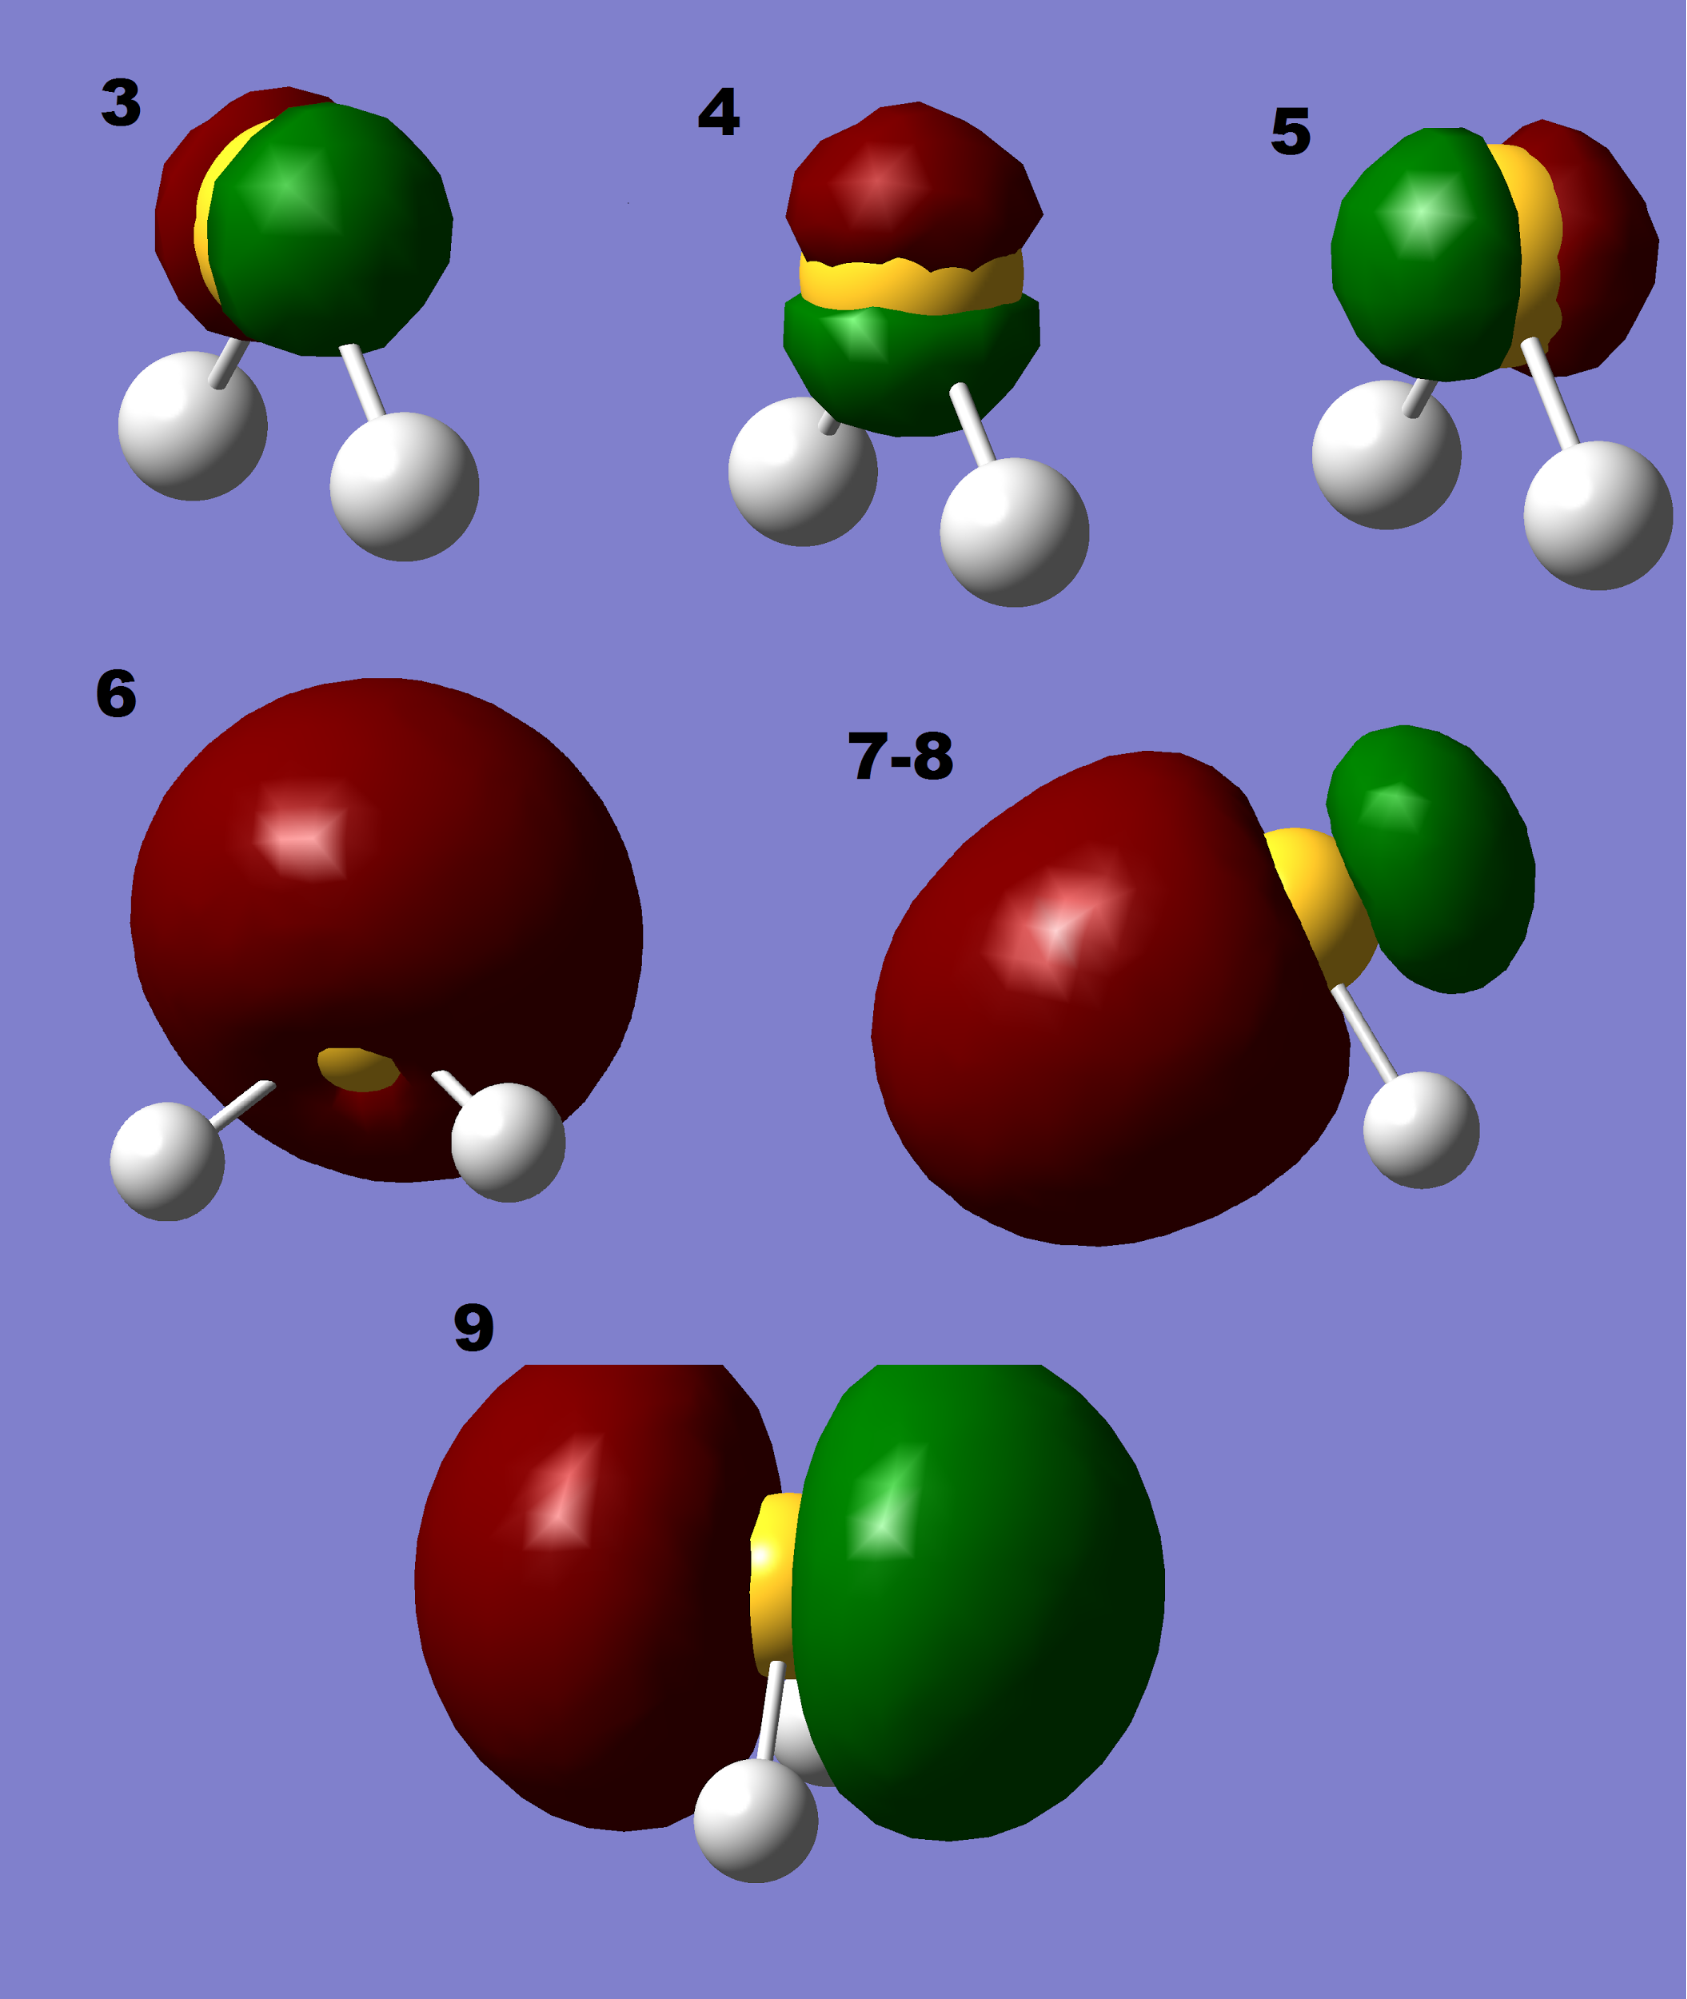
\includegraphics{images/image4.png}}

{Figura 4: }{Diagrama de los orbitales naturales con el método
RHF/3-21g, donde los orbitales 3,4 y 5 son de Core. El orbital 6 y 9 son
Lone Pairs, que corresponde a los pares libres en la estructura de
Lewis. Los orbitales 7 y 8, solo graficado uno porque son simétricos,
son finalmente los orbitales enlazantes o }{bonding}

{}

\protect\hypertarget{t.699ec4088e819c261a6f6322d85d42212259f0cf}{}{}\protect\hypertarget{t.7}{}{}

\begin{longtable}[]{@{}llll@{}}
\toprule
\begin{minipage}[t]{0.22\columnwidth}\raggedright\strut
{Orbital}\strut
\end{minipage} & \begin{minipage}[t]{0.22\columnwidth}\raggedright\strut
{Tipo}\strut
\end{minipage} & \begin{minipage}[t]{0.22\columnwidth}\raggedright\strut
{Ocupación}\strut
\end{minipage} & \begin{minipage}[t]{0.22\columnwidth}\raggedright\strut
{Energía}\strut
\end{minipage}\tabularnewline
\begin{minipage}[t]{0.22\columnwidth}\raggedright\strut
{3}\strut
\end{minipage} & \begin{minipage}[t]{0.22\columnwidth}\raggedright\strut
{CR}\strut
\end{minipage} & \begin{minipage}[t]{0.22\columnwidth}\raggedright\strut
{1,99922 ~ ~}\strut
\end{minipage} & \begin{minipage}[t]{0.22\columnwidth}\raggedright\strut
{-8,78321}\strut
\end{minipage}\tabularnewline
\begin{minipage}[t]{0.22\columnwidth}\raggedright\strut
{4}\strut
\end{minipage} & \begin{minipage}[t]{0.22\columnwidth}\raggedright\strut
{CR}\strut
\end{minipage} & \begin{minipage}[t]{0.22\columnwidth}\raggedright\strut
{2,0000}\strut
\end{minipage} & \begin{minipage}[t]{0.22\columnwidth}\raggedright\strut
{-6,58774}\strut
\end{minipage}\tabularnewline
\begin{minipage}[t]{0.22\columnwidth}\raggedright\strut
{5}\strut
\end{minipage} & \begin{minipage}[t]{0.22\columnwidth}\raggedright\strut
{CR}\strut
\end{minipage} & \begin{minipage}[t]{0.22\columnwidth}\raggedright\strut
{1,99983}\strut
\end{minipage} & \begin{minipage}[t]{0.22\columnwidth}\raggedright\strut
{-6,59035}\strut
\end{minipage}\tabularnewline
\begin{minipage}[t]{0.22\columnwidth}\raggedright\strut
{6}\strut
\end{minipage} & \begin{minipage}[t]{0.22\columnwidth}\raggedright\strut
{LP}\strut
\end{minipage} & \begin{minipage}[t]{0.22\columnwidth}\raggedright\strut
{2,00000 ~ ~}\strut
\end{minipage} & \begin{minipage}[t]{0.22\columnwidth}\raggedright\strut
{-0,83012}\strut
\end{minipage}\tabularnewline
\begin{minipage}[t]{0.22\columnwidth}\raggedright\strut
{7}\strut
\end{minipage} & \begin{minipage}[t]{0.22\columnwidth}\raggedright\strut
{BD}\strut
\end{minipage} & \begin{minipage}[t]{0.22\columnwidth}\raggedright\strut
{1,99852}\strut
\end{minipage} & \begin{minipage}[t]{0.22\columnwidth}\raggedright\strut
{-0,76027}\strut
\end{minipage}\tabularnewline
\begin{minipage}[t]{0.22\columnwidth}\raggedright\strut
{8}\strut
\end{minipage} & \begin{minipage}[t]{0.22\columnwidth}\raggedright\strut
{BD}\strut
\end{minipage} & \begin{minipage}[t]{0.22\columnwidth}\raggedright\strut
{1,99852}\strut
\end{minipage} & \begin{minipage}[t]{0.22\columnwidth}\raggedright\strut
{-0,76027}\strut
\end{minipage}\tabularnewline
\begin{minipage}[t]{0.22\columnwidth}\raggedright\strut
{9}\strut
\end{minipage} & \begin{minipage}[t]{0.22\columnwidth}\raggedright\strut
{LP}\strut
\end{minipage} & \begin{minipage}[t]{0.22\columnwidth}\raggedright\strut
{2,00000 ~ ~}\strut
\end{minipage} & \begin{minipage}[t]{0.22\columnwidth}\raggedright\strut
{-0,39732}\strut
\end{minipage}\tabularnewline
\bottomrule
\end{longtable}

{Tabla 8:}{~Ocupación, tipo y energía de los orbitales naturales de la
Figura 4, obtenidos del método RHF/3-21g.}

{}

\protect\hypertarget{t.2dff5057e1400861e8aca07e8a18d6d69613d450}{}{}\protect\hypertarget{t.8}{}{}

\begin{longtable}[]{@{}llll@{}}
\toprule
\begin{minipage}[t]{0.22\columnwidth}\raggedright\strut
{Atomo}\strut
\end{minipage} & \begin{minipage}[t]{0.22\columnwidth}\raggedright\strut
{Nro}\strut
\end{minipage} & \begin{minipage}[t]{0.22\columnwidth}\raggedright\strut
{Carga natural {[}e}{-}{{]}}\strut
\end{minipage} & \begin{minipage}[t]{0.22\columnwidth}\raggedright\strut
{Carga Mulliken {[}e}{-}{{]}}\strut
\end{minipage}\tabularnewline
\begin{minipage}[t]{0.22\columnwidth}\raggedright\strut
{S}\strut
\end{minipage} & \begin{minipage}[t]{0.22\columnwidth}\raggedright\strut
{1}\strut
\end{minipage} & \begin{minipage}[t]{0.22\columnwidth}\raggedright\strut
{-0}{,}{26645}\strut
\end{minipage} & \begin{minipage}[t]{0.22\columnwidth}\raggedright\strut
{-0}{,}{1581}{8}{~ }\strut
\end{minipage}\tabularnewline
\begin{minipage}[t]{0.22\columnwidth}\raggedright\strut
{H}\strut
\end{minipage} & \begin{minipage}[t]{0.22\columnwidth}\raggedright\strut
{2}\strut
\end{minipage} & \begin{minipage}[t]{0.22\columnwidth}\raggedright\strut
{0}{,}{13323}\strut
\end{minipage} & \begin{minipage}[t]{0.22\columnwidth}\raggedright\strut
{0}{,}{0790}{9}\strut
\end{minipage}\tabularnewline
\begin{minipage}[t]{0.22\columnwidth}\raggedright\strut
{H}\strut
\end{minipage} & \begin{minipage}[t]{0.22\columnwidth}\raggedright\strut
{3}\strut
\end{minipage} & \begin{minipage}[t]{0.22\columnwidth}\raggedright\strut
{0}{,}{13323}\strut
\end{minipage} & \begin{minipage}[t]{0.22\columnwidth}\raggedright\strut
{0}{,}{0790}{9}\strut
\end{minipage}\tabularnewline
\bottomrule
\end{longtable}

{Tabla 9}{: Carga natural versus carga Mulliken, obtenidas por el método
RHF/3-21g}

{}

\protect\hypertarget{t.89d0007008d0fd90d12bdec7c4c69a3f3ff6fa71}{}{}\protect\hypertarget{t.9}{}{}

{Dipolo natural}

{Dipolo Mulliken}

{x{[}D{]}}

{y{[}D{]}}

{z{[}D{]}}

{x{[}D{]}}

{y{[}D{]}}

{z{[}D{]}}

{0}

{0}

{-}{1,8100}

{0}

{0}

{-1,8103}

{Tabla 10: }{Dipolo natural versus dipolo Mulliken, obtenidas con el
método RHF/3-21g}

{}

{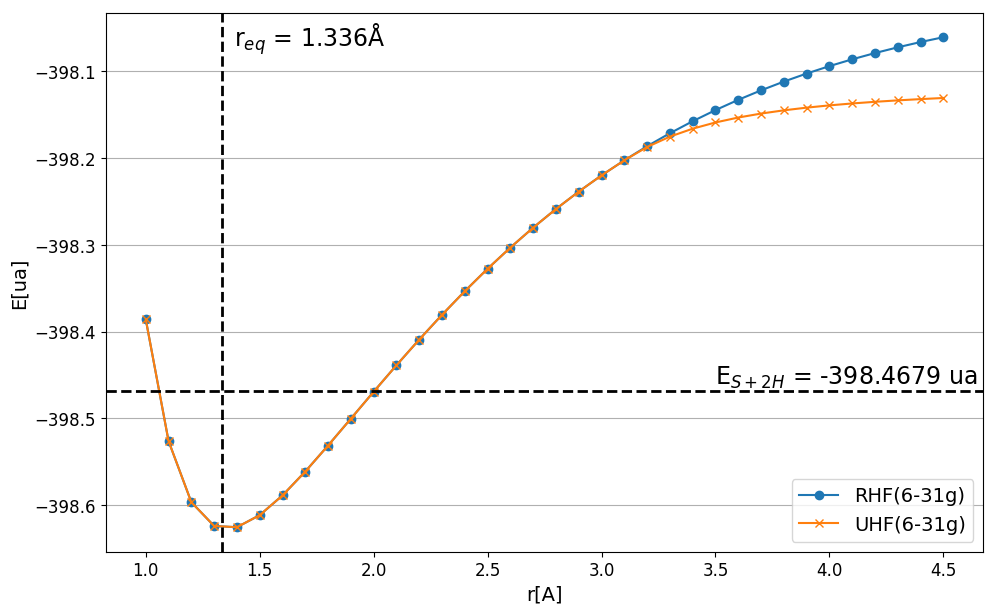
\includegraphics{images/image7.png}}

{Figura 5: }{Energía de la molécula versus ~distancia H-S para la
molécula H}{2}{S con ~método RHF y UHF, base 6-31G. La línea horizontal
representa la energía de S + 2H por el método RHF/6-31g, mientras que la
línea vertical es la distancia de equilibrio experimental de la
molécula. }

{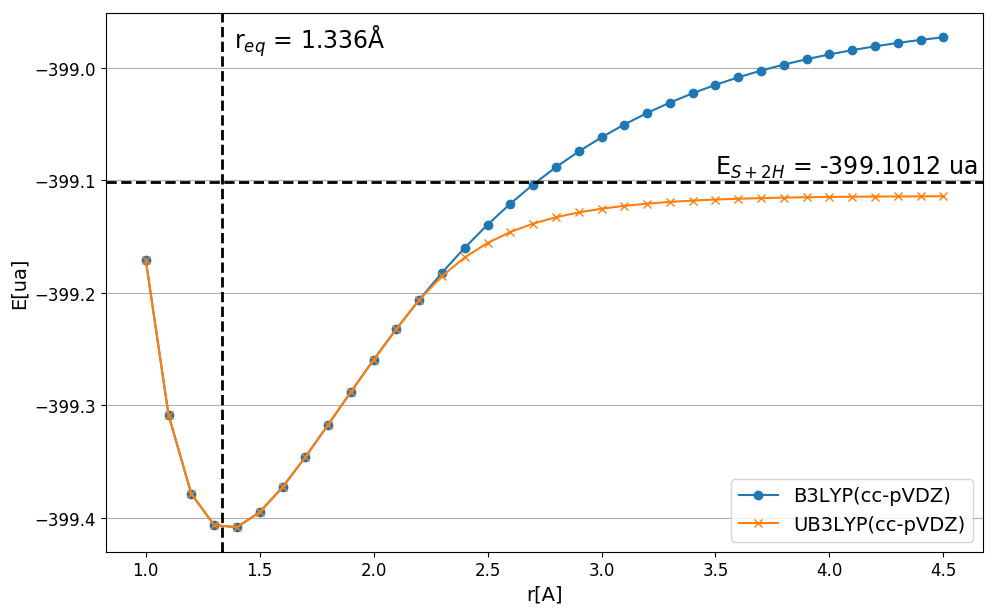
\includegraphics{images/image3.png}}

{Figura 6: ~}{Energía de la molécula versus ~distancia H-S para la
molécula H}{2}{S con el método B3LYP y UB3LYP, base cc-pVDZ. Se observa
la diferencia entre el método restricto e irrestricto, a una menor
distancia que para el ~cálculo con HF. Además el método irrestricto
describe correctamente la energía de los átomos totalmente disociados}

{}

{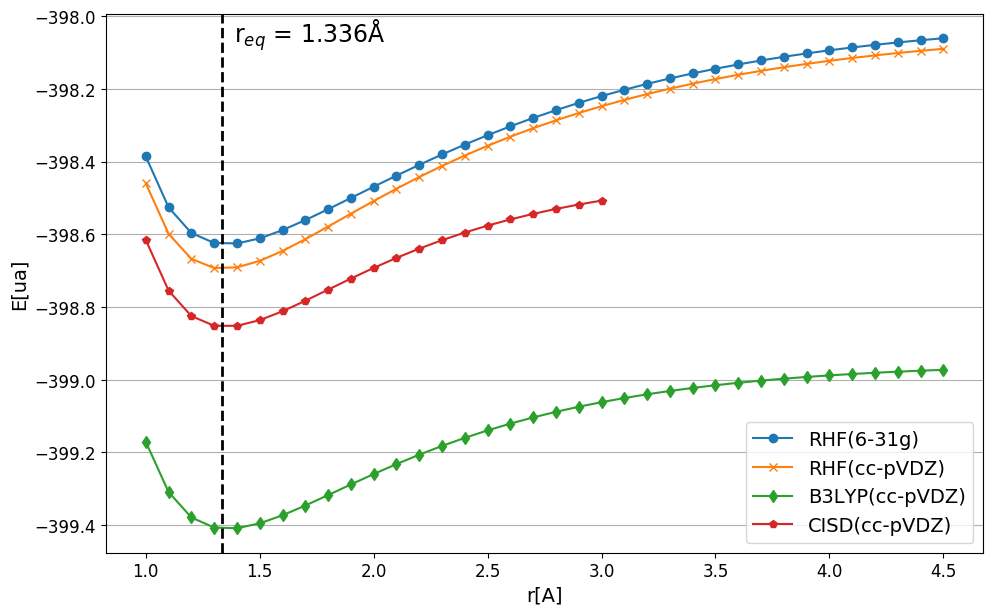
\includegraphics{images/image6.png}}

{Figura 7}{: }{~}{Energía de la molécula versus ~distancia H-S para la
molécula H}{2}{S ~con ~diferentes métodos en el caso restricto. La
distancia de equilibrio experimental se grafica en la línea vertical
punteada para comparar el equilibrio de cada método}

{}

\end{document}
